 %%%%%%%%%%%%%%%%%%%%%%%%%%%%%%%%%%%%%%%%%%%%%%%%%%%%%%%%%%%%%%%%%%%%%%
% LaTeX Example: Project Report
%
% Source: http://www.howtotex.com
%
% Feel free to distribute this example, but please keep the referral
% to howtotex.com
% Date: March 2011 
% 
%%%%%%%%%%%%%%%%%%%%%%%%%%%%%%%%%%%%%%%%%%%%%%%%%%%%%%%%%%%%%%%%%%%%%%
% How to use writeLaTeX: 
%
% You edit the source code here on the left, and the preview on the
% right shows you the result within a few seconds.
%
% Bookmark this page and share the URL with your co-authors. They can
% edit at the same time!
%
% You can upload figures, bibliographies, custom classes and
% styles using the files menu.
%
% If you're new to LaTeX, the wikibook is a great place to start:
% http://en.wikibooks.org/wiki/LaTeX
%
%%%%%%%%%%%%%%%%%%%%%%%%%%%%%%%%%%%%%%%%%%%%%%%%%%%%%%%%%%%%%%%%%%%%%%
% Edit the title below to update the display in My Documents
%\title{Project Report}
%
%%% Preamble
\documentclass[paper=a4, fontsize=11pt]{scrartcl}
\usepackage[T1]{fontenc}
\usepackage{fourier}
\usepackage{tabularx}
\usepackage[utf8]{inputenc}
\usepackage{hyperref}

\usepackage{graphicx}
\usepackage{caption}
\usepackage{subcaption}

\usepackage[english]{babel}															% English language/hyphenation
\usepackage[protrusion=true,expansion=true]{microtype}	
\usepackage{amsmath,amsfonts,amsthm} % Math packages

\usepackage{url}
%\usepackage[hang, small,labelfont=bf,up,textfont=it,up]{caption}


%%% Custom sectioning
\usepackage{sectsty}
\allsectionsfont{\normalfont\scshape}
\usepackage{float}
\usepackage{amsmath}
\usepackage{mathtools}



%%% Custom headers/footers (fancyhdr package)
\usepackage{fancyhdr}
\pagestyle{fancyplain}
\fancyhead{}											% No page header
\fancyfoot[L]{}											% Empty 
\fancyfoot[C]{}											% Empty
\fancyfoot[R]{\thepage}									% Pagenumbering
\renewcommand{\headrulewidth}{0pt}			% Remove header underlines
\renewcommand{\footrulewidth}{0pt}				% Remove footer underlines
\setlength{\headheight}{13.6pt}


%%% Equation and float numbering
\numberwithin{equation}{section}		% Equationnumbering: section.eq#
\numberwithin{figure}{section}			% Figurenumbering: section.fig#
\numberwithin{table}{section}				% Tablenumbering: section.tab#


%%% Maketitle metadata

\newcommand{\horrule}[1]{\rule{\linewidth}{#1}} 	% Horizontal rule

\title{
		%\vspace{-1in} 	
		\usefont{OT1}{bch}{b}{n}
		\normalfont \normalsize \textsc{} \\ [25pt]
		
\includegraphics[width=0.5\linewidth]{sno} \\
		
\includegraphics[width=0.4\linewidth]{tru}		
		\horrule{0.5pt} \\[0.2cm]
		\huge Umbilical Retrieval Mechanism Work Report \\
		\horrule{2pt} \\[0.005cm]
}
\author{
		\normalfont 								\normalsize
        Jerin Roberts\\[-5pt]		\normalsize
        \today
}
\date{}




%%% Begin document
\begin{document}
\maketitle
\begin{center}
\begin{tabular}{l r}


Supervisors: & Dr. Christine Kraus, Dr. Erica Caden  \\ % supervisor
Locations: & SNOLAB, Laurentian University


\end{tabular}
\end{center}
\newpage
\tableofcontents
\listoffigures
\listoftables
\newpage

\section{Introduction}

This report is a summary of the work completed on the umbilical retrieval mechanism (URM) during the summer work period of (May to August 2014). The summary of my work includes reducing and quantifying slippage of the URM drive system. Descriptions of the component modifications as well as the methods for data collection are described in this report.

\section{Umbilical Retrieval Mechanism}
\subsection{Overview}

The umbilical retrieval mechanism (URM)is a device that is used to deploy and store an umbilical for source connections for the SNO+ experiment. The device, as displayed in figure \ref{av} sits on the glove port on top of the SNO+ detector. The URM enables the communication between sources and the deck when they are lowered into the acrylic vessel (AV) during calibrations of both the water and scintillation phases of the SNO+ experiment.
\begin{figure}[h!]
\centering
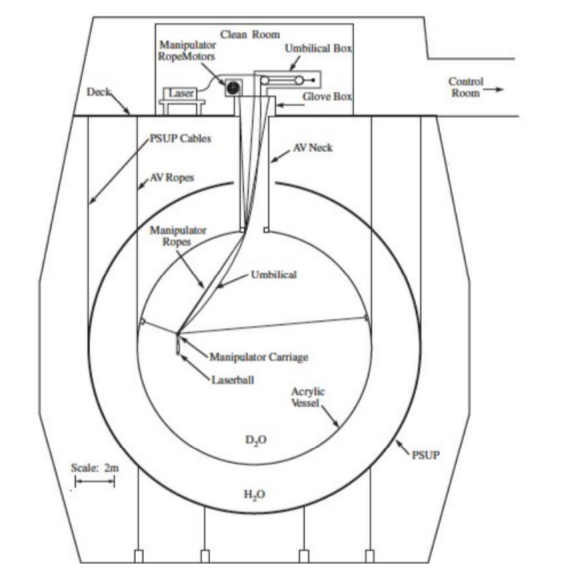
\includegraphics[width=0.5\linewidth]{avdia}
\caption{Displays a diagram of the SNO+ detector. The URM is shown sitting on top of the glove box inside the deck clean room (DCR) \cite{picfsk}}
\label{av}
\end{figure} 
\subsection{Umbilical}
The umbilical which is deployed by the URM is used to communicate with calibration sources for SNO+. The umbilical contains a number of hook-up wires, a coaxial cable and a core designed to house fibre lines. Shown in figure \ref{umb} is a display of its internal structure. Previous umbilical lines used for SNO where constructed using an external silicon tube. 
\begin{figure}[h!]
\centering
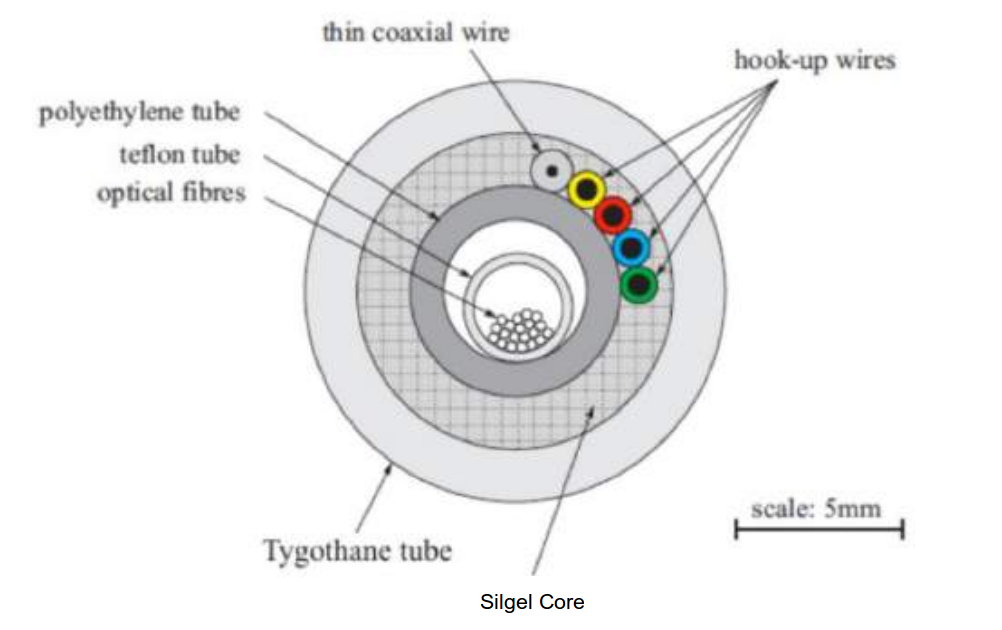
\includegraphics[width=0.65\linewidth]{umb}
\caption{Displays a cross-section schematic of the umbilical planned for SNO+. \cite{picfsk}}
\label{umb}
\end{figure}
 In SNO+, the exterior consists of a Tygothane tube with a SilGel 612 or ClearFlex 50 internal gel which is used for compatibility with linear alkyl-benzene (LAB) during scintillation phase \cite{picfsk}. Umbilical construction and tests continue at Queens university.
\subsection{Drive Assembly}
The drive-assembly on the URM is the main device which extends and retracts the umbilical. The free floating device comprises of a system of pulleys which guide the umbilical onto the drive pulley. The guide pulleys swivel on a spring-loaded swing-arm system which allows for the application of a continuous pinch force between the main and guide pulleys. The entire system, which is displayed in figure \ref{dr} swivels from a single pivot and is suspended at the opposite end using a load cell. This enables the measure of the tension exerted onto the drive umbilical during deployment operations. 


\begin{figure}[h]
        \centering
        \begin{subfigure}[h]{0.8\textwidth}
                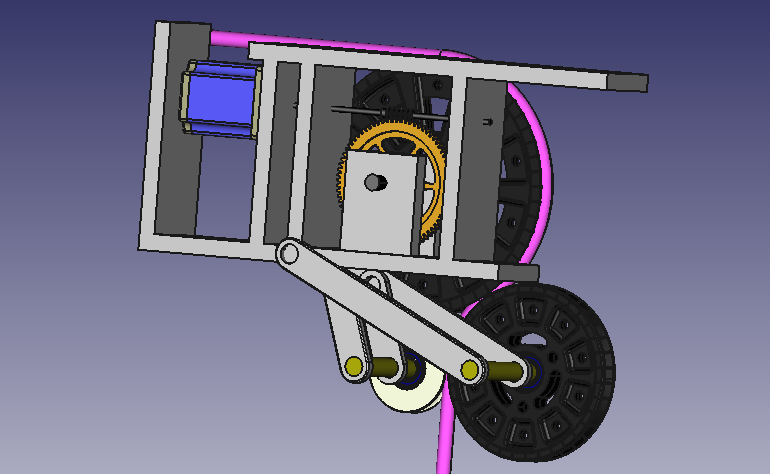
\includegraphics[height = 5cm]{original1}
                \caption{}
				
        \end{subfigure}%
       \quad
        \begin{subfigure}[h]{0.8\textwidth}
                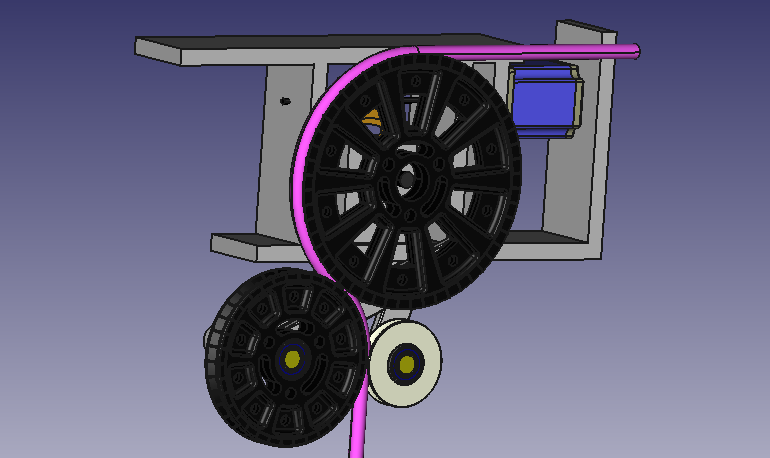
\includegraphics[height = 5cm]{original2}
                \caption{}
                
        \end{subfigure}
        \quad

        \caption{Displays the drive assembly component of the URM generated using FreeCAD 3D modeller.}
        \label{dr}
\end{figure}

The in addition the assembly also houses the stepper motor which drives the main pulley via a gear/spiral cog reduction.The stepper motor and other sensors, are run on Ubuntu 12.04 via the MANIP program. The $ChangePos$ command is used to primitively extend and retract the umbilical. The length of the umbilical extended and retracted during experimental operations is measured using a rotary optical encoder which is mounted on the top of the drive assembly shown in figure \ref{dr2}. The encoder readout is accessible through the $read$ or $readloop$ command. 

\subsection{Storage System}
During the operation of deployment the excess umbilical is spooled in the storage area as displayed in figure \ref{hhh}. The storage mechanism consists of both a stationary pulley block and floating block tensioned via a pneumatic cylinder. The umbilical is wrapped several times around these pulleys before exiting the URM. When the umbilical is retracted the tensioned block takes up the excess umbilical being driven into the storage area. When extending the storage mechanism releases the umbilical under tension which keeps the excess spooled on the pulley blocks \cite{p1}.

\begin{figure}[h]
        \centering
        \begin{subfigure}[h]{0.8\textwidth}
                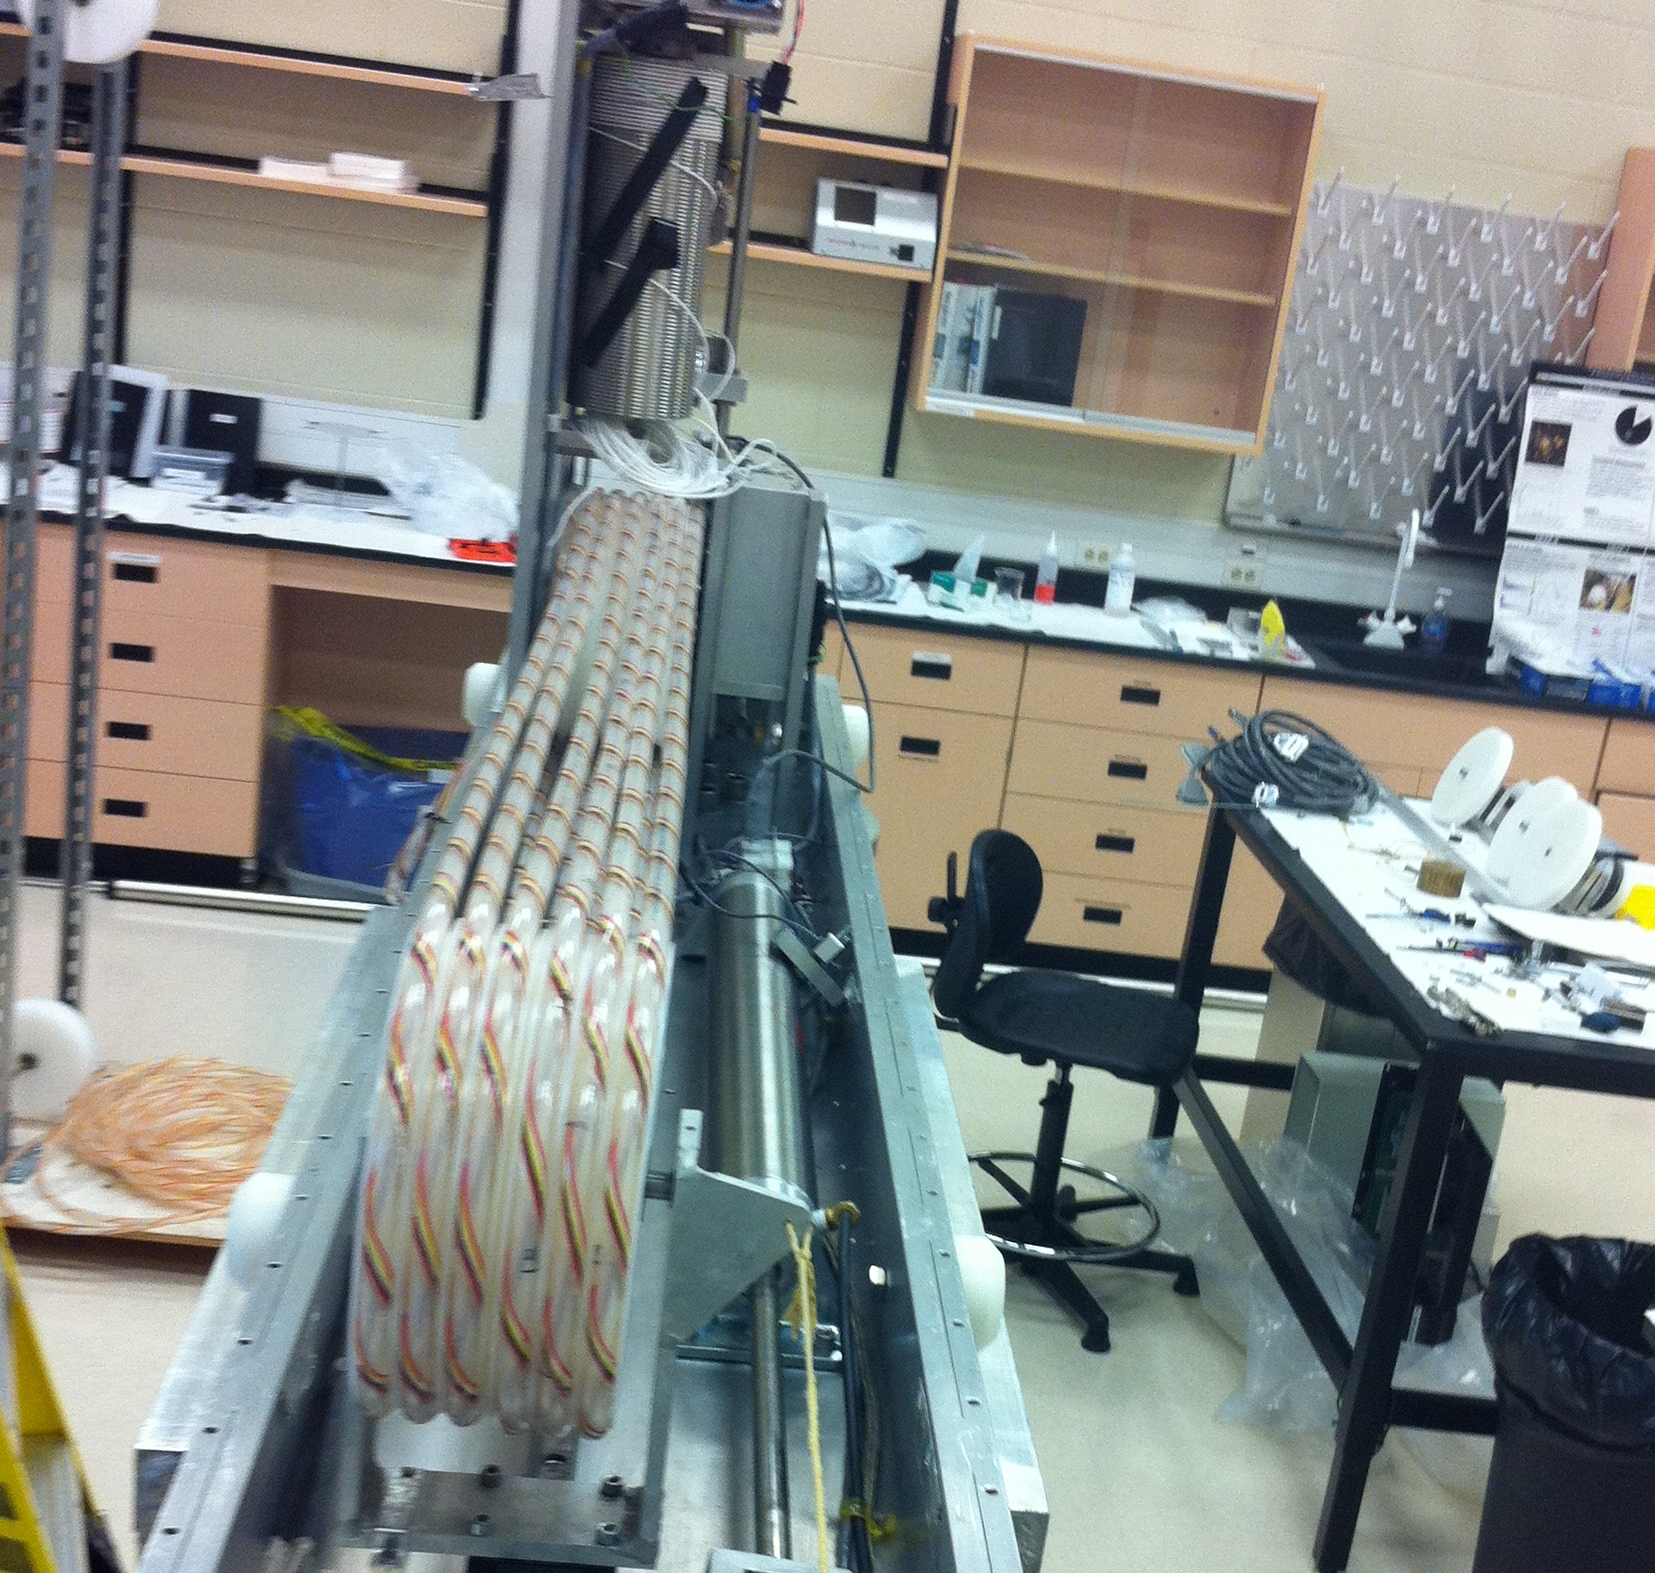
\includegraphics[height = 5cm]{hhh1}
                \caption{}
				
        \end{subfigure}%
       \quad
        \begin{subfigure}[h]{0.8\textwidth}
                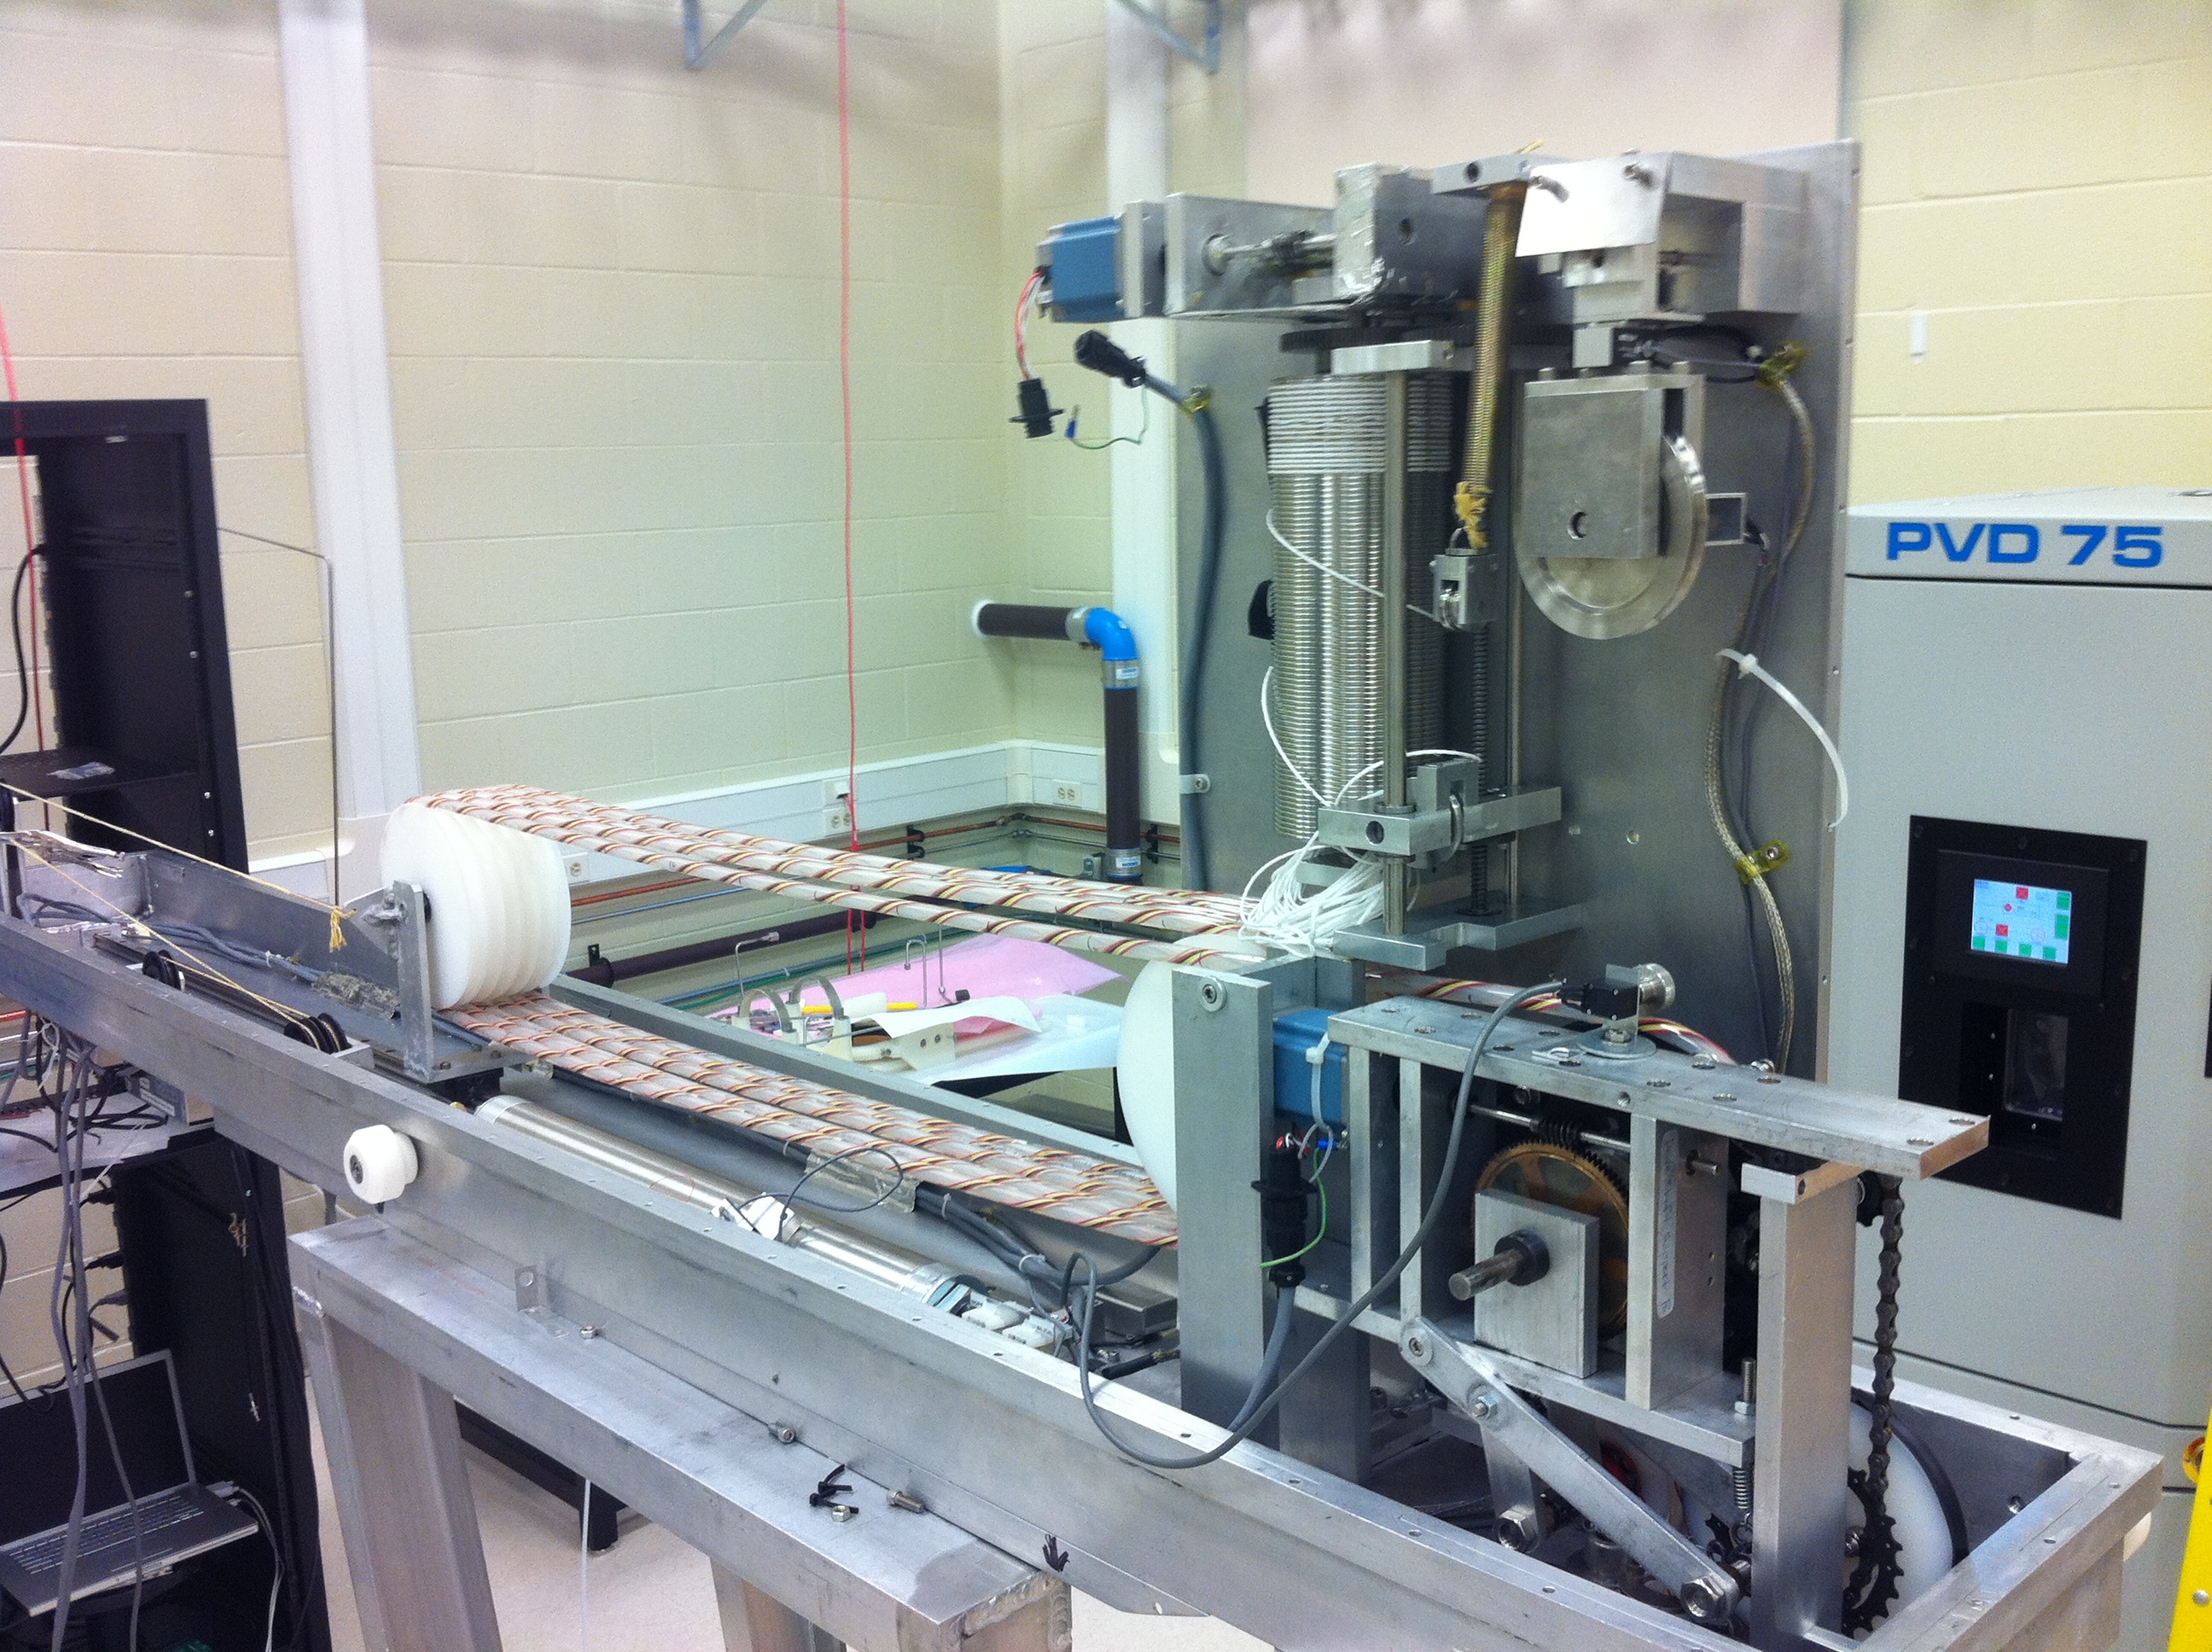
\includegraphics[height = 5cm]{hhh2}
                \caption{}
                \label{dr2}
        \end{subfigure}
        \quad

        \caption{Displays the drive assembly component of the URM.}
        \label{hhh}
\end{figure}
The air pressure that activates the pneumatic cylinder is supplied via a compressed air line and a pressure regulator. 
\section{URM Modifications}
\subsection{Slippage Sources}
The URM will be responsible for source deployment for both water and scintillation phases of the SNO+ experiment. A new URM design is required during the scintillation phase for LAB compatibility and background requirements. Linear Alkyl-Benzene is an organic mineral oil with a low coefficient of friction. This compounding with the slippery tygothane tubing causes major slippage on the main drive pulley. The designed of the main drive pulley is also inherently susceptible to slippage through its smooth half moon track design. In addition to major slippage issues there existed an asymmetry between the extend and retraction modes of operation. This is caused by the pneumatic cylinder which tensions the deploying umbilical. Essentially this system causes significantly more slippage to occur during extension operations.
\subsection{Pulley Design}
The track of the main drive pulley was redesigned and modified by Lawrence Garcia. His 46 degree V-slot design (figure \ref{pul2}) with aggressively raised tread was implemented on the redesign of both the main and big guide pulleys. The pulleys in order to reduced warping and manufacture costs are printed in two pieces then fastened together axially using bolts. The original prototype pulley, built by Garcia, due to width requirements had to be shaved down, which ultimately reduced the strength in the fastening mounts which caused them to fail. The new pulleys were redesigned with stronger fastening mounts and fillet edges to reduce concentrating stresses at sharp points. The aggressive V-slot concept was also implemented into the big guide pulley design. The new pulleys where printed and mounted, which are displayed in figure \ref{pul1}

\begin{figure}[h]
        \centering
        \begin{subfigure}[h]{0.8\textwidth}
                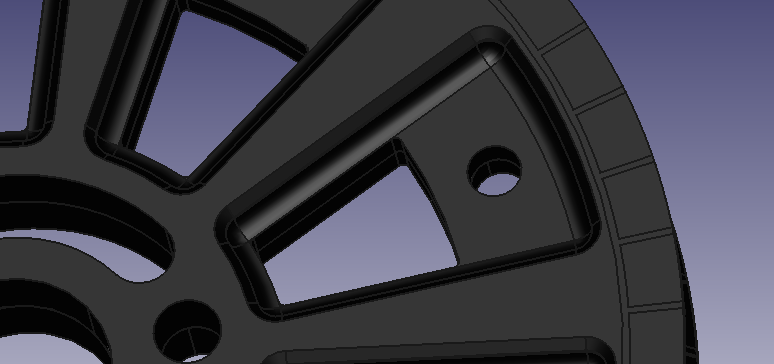
\includegraphics[height=5cm]{pull2}
                \caption{}
				\label{pul3}
        \end{subfigure}%
       \quad
        \begin{subfigure}[h]{0.8\textwidth}
                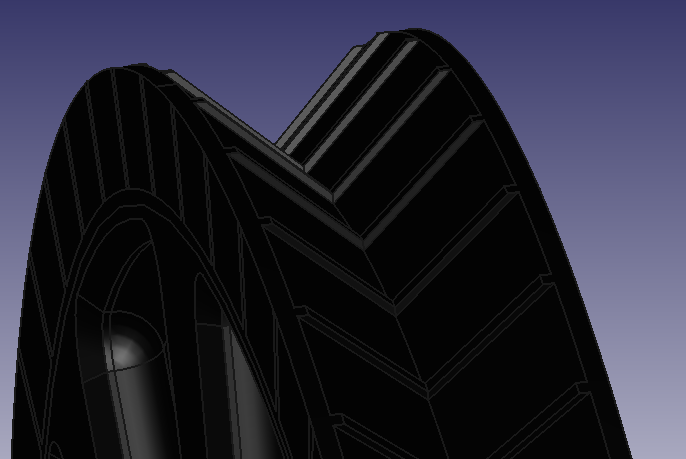
\includegraphics[height=7cm]{pull3}
                \caption{}
                \label{pul2}
        \end{subfigure}
        \quad

        \caption{Displays the new pulleys designs for the URM.}
        \label{pul1}
\end{figure}
Finite element method (FEM) is a numerical technique for finding approximate solutions to boundary value problems for partial differential equations (PDE's) and is implemented in FEM analysis software. Calculus of variations is used to minimize an error function and produce a stable solution. The partial DE solved usually describes the physics of interest in the FEM simulation. For example when simulating fluid flow, the PDE solved, may be a variation of the Navier-Stokes equation.
The Pulleys design were validated using a Linux FEM analyser called Z88Aurora. This software was used to compare the relative rigidity of the new pulleys. An example of the analysis is shown in figure \ref{fem1} which compares the stresses between the original and new rounded design. Figures \ref{fema} and \ref{femc} display the stresses formed on new fillet design while figures \ref{femb} and \ref{femd} show the original sharp corner design using typical load geometries.
Although the simulation was relative, this was a basic analysis using a linear tetrahedron model for polyoxymethylene (POM), which allowed us to validate that the new structural design would more evenly distribute the stresses experienced. The New Main and Guide pulleys designs contributed to the overall slippage reduction during URM operations
\begin{figure}[H]
        \centering
        \begin{subfigure}[h]{0.8\textwidth}
                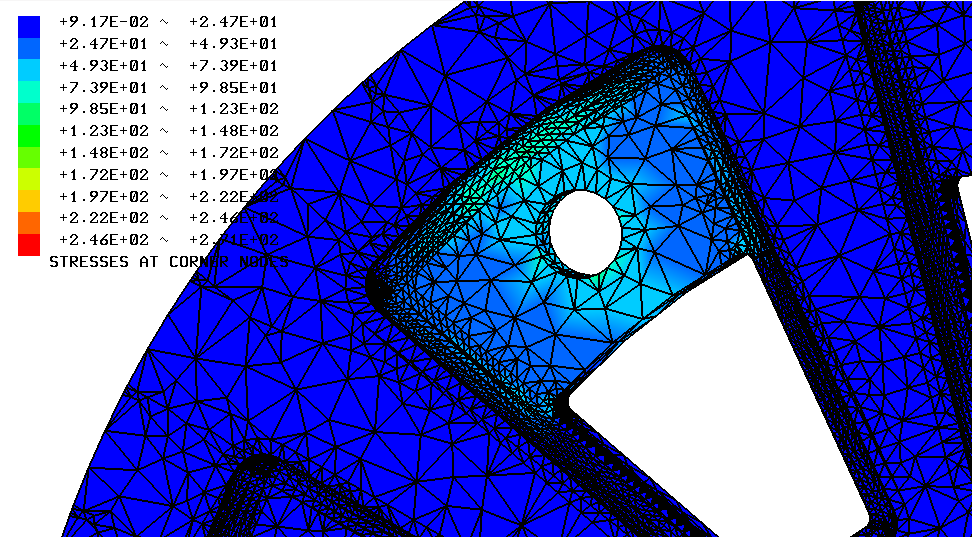
\includegraphics[height=5cm]{good502}
                \caption{}
				\label{fema}
        \end{subfigure}%
       \quad
        \begin{subfigure}[h]{0.8\textwidth}
                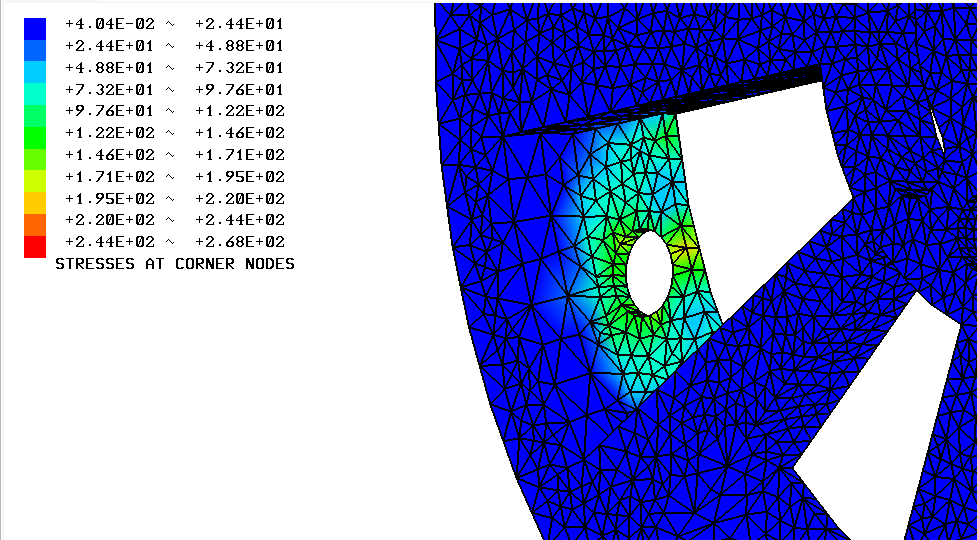
\includegraphics[height=5cm]{goodorig502}
                \caption{}
                \label{femb}
        \end{subfigure}
        
         \begin{subfigure}[h]{0.8\textwidth}
                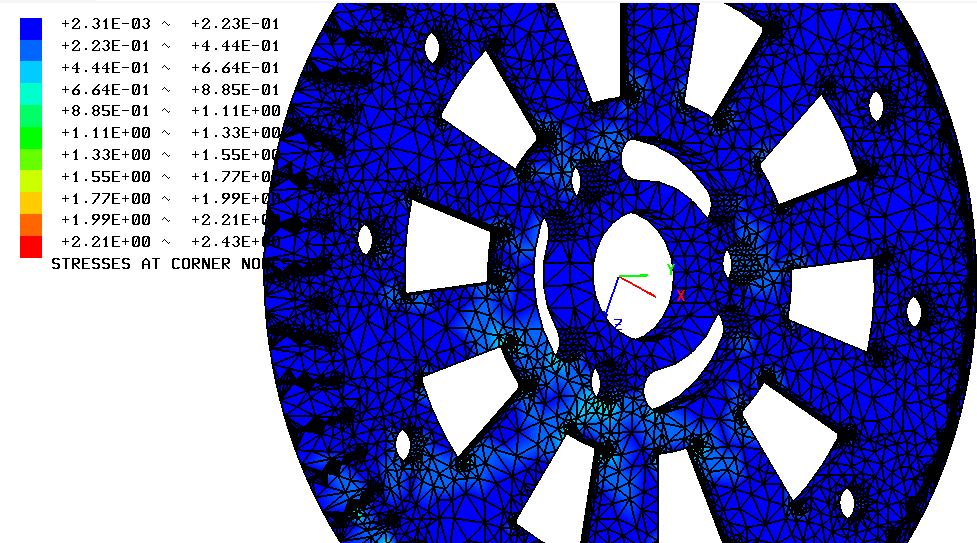
\includegraphics[height=5cm]{rotationnew1}
                \caption{}
				\label{femc}
        \end{subfigure}%
       \quad
        \begin{subfigure}[h]{0.8\textwidth}
                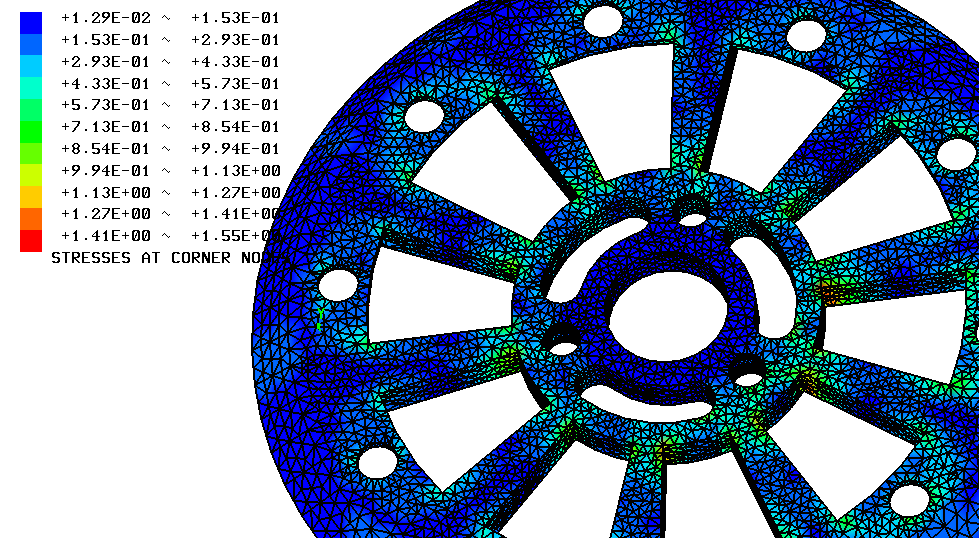
\includegraphics[height=5cm]{rotationoriginal1}
                \caption{}
                \label{femd}
        \end{subfigure}
        \quad

        \caption{FEM analysis of both the original and redesigned drive pulley; The top row simulates axial loads, while the bottom simulates equatorial and radial loads.}
        \label{fem1}
\end{figure}

\subsection{Chain Drive System}
In the original drive assembly only the main pulley was driven by the stepper motor. In order to reduce slippage a chain drive system was implemented to drive the remaining guide pulleys. The system contains common bicycle components and was implemented to test the feasible improvements that could be made through driving the additional guide pulleys. The idea enables a more efficient use of the force provided by the spring-loaded swing-arms and effectively reduces the slippage on the main pulley. Figure \ref{chd} shows a diagram of the design implemented. 

\begin{figure}[h]
        \centering
        \begin{subfigure}[h]{0.8\textwidth}
                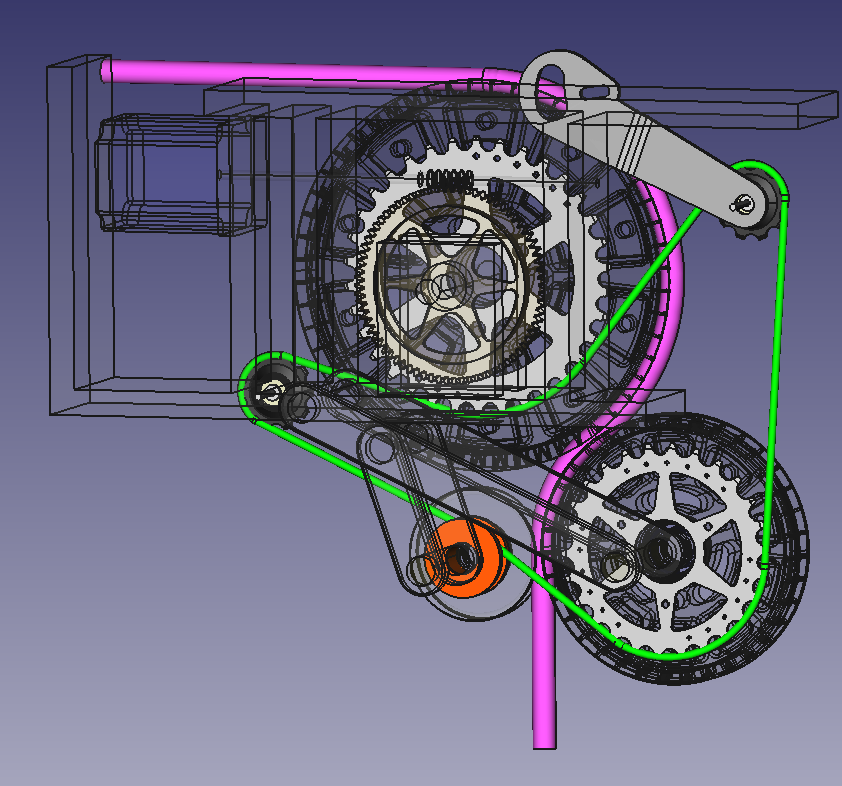
\includegraphics[height=6cm]{final3}
                \caption{}
				\label{chd1}
        \end{subfigure}%
       \quad
        \begin{subfigure}[h]{0.8\textwidth}
                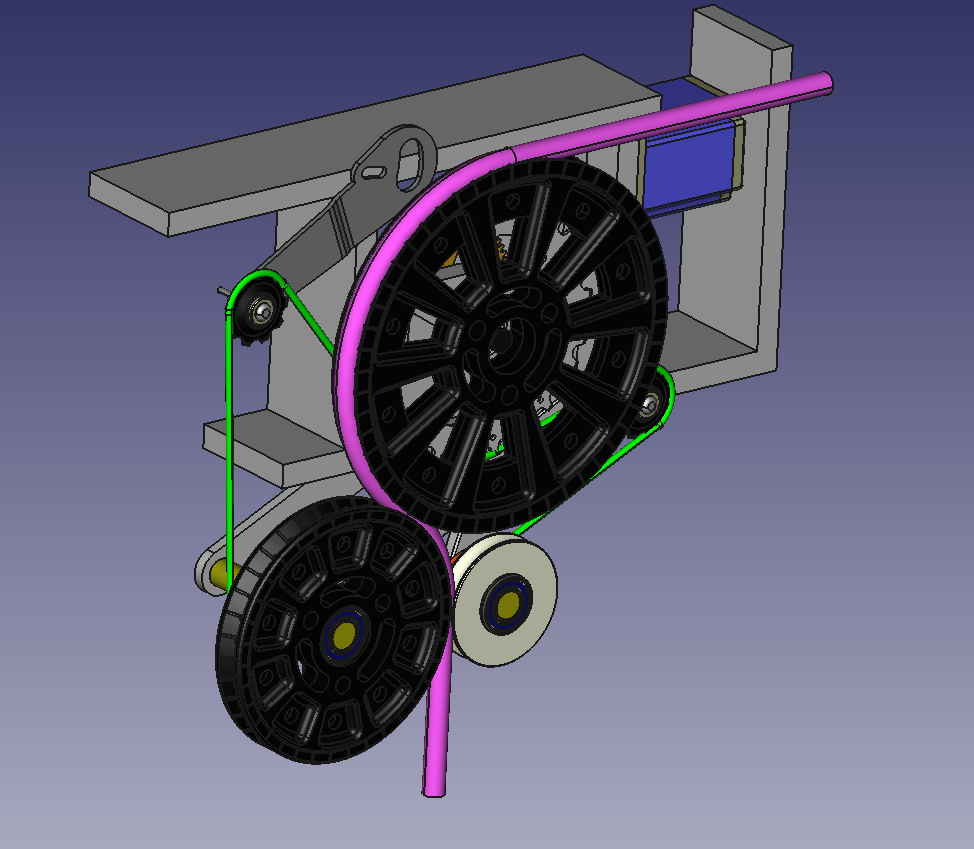
\includegraphics[height=6cm]{final1}
                \caption{}
                \label{chd2}
        \end{subfigure}
        \quad

        \caption{Displays the drive assembly component of the URM.}
        \label{chd}
\end{figure}
The system was designed to be low cost and easily implemented with little modification to the original URM. The system consists of sprockets mounted on the pulleys and driven by a guided chain. The sprockets are chosen to specifically match the ratio between the radii of the umbilical as it sits on the pulleys. This ensures a proper gear ratio between the sprockets and ensures smooth meshing of the pulleys at the umbilical to pulley interface. The gear ratio used between the main and guide pulley respectfully was 1.487:1. A static Tensioner is used to adjust tension on the chain, while a chain guide is currently used in place of a sprocket on the small guide pulley. The chain line has been chosen for easy future attachment of a sprocket to the small guide pulley which would require a ratio of 2.05:1 between the big guide and small guide pulley respectively.
\section{Data}
\subsection{Method}
The slippage was measured using a conventional ruler with mm increments and validated using the rotary optical encoder. The umbilical was extended and retracted using the ChangePos (-) and (+) respectively. The actual deployed length is then compared to the requested ChangePos length. The difference found between the two represents the slippage experience during the run. In order to attain accurate slippage measurements the steps per unit length value in the MOTOR.DAT file was adjusted. The amount of umbilical contained on half the pulley was measured and doubled. This circumference value was then entered as a ChangePos command. The steps/unit length was then adjusted until the pulley would complete a full revolution during this specific command. The value could be further refined by multiplying the encircling ChangePos value by 'n' times and validating the completion of 'n' revolutions during this command. 

\begin{table}[H]
\begin{tabularx}{\textwidth}{ |X|X|X|X|X|X| }
\hline
ChangePos  & Initial  & Extended  & Retracted  & Slippage  & Slippage \\ 
 (+-) & Position & Position & Position & Extended & Retracted \\
\hline
50cm &	 207.5cm & 	255cm & 	206.5cm &	5.00\%  &	3.00 \%	
 \\
\hline
100cm &	206.5cm	& 301.3cm	& 204cm &	5.20\% & 	2.70\%	\\
\hline

\end{tabularx}
\caption{Displays a data sample }
\label{data}
\end{table}

This method resulted in a steps per unit length value of 305 steps/cm. A typical data run is completed as follows; The initial position of the umbilical is recorded, a changepos (-) command is run and the resulting position is measured, a changepos (+) command is then run and the final position is measured and recorded. Using these points the percent slippage for both extension and retraction are calculated. A collection sample is displayed in table \ref{data}.
\subsection{Measured Slippage}
Figure \ref{fit1} and \ref{fit2} display measured extension and retraction values versus the requested length change. The slope of the line represents the actual travelled decimal percentage. Or more specifically the umbilical will only deploy 95\% of the requested length. Figure \ref{fit1} contrasts the results from both the non-chain and chain drive systems. In addition the graph also demonstrates the asymetry seen between the extension and retraction phases for the non-chain drive system. The blue line (figure \ref{fit1}) shows the improvements made by the addition of the chain drive system. The graph in figure \ref{fit2} demonstrates the linearity of the measured slippage for both short and long ChangePos commands. This was further validated by calculating a coefficient of determination for the data.


   

     


The coefficient of determination ($R^2$) which in this case denotes the linearity of the fitted data, was calculated using equation \ref{eq} where the value of $y_i$ represents an independent variable, $f_i$ is the fitted function, and $\bar{y}$ is the mean of the data set. 

\begin{equation}
\label{eq}
R^2=1-\frac{\sum\limits_{i} (y_i-f_i)^2}{\sum\limits_{i} (y_i-\bar{y})^2}
\end{equation}

A value of 1.00 would represent a perfect fit and in this case perfectly linear data set. The coefficient of determination for figure \ref{fit2} was found to be 0.9978. The slope of line of best fit was calculated using ROOT and was found to be 0.9582$\pm$0.0029$\frac{cm}{cm}$.

     \begin{figure}[H]
                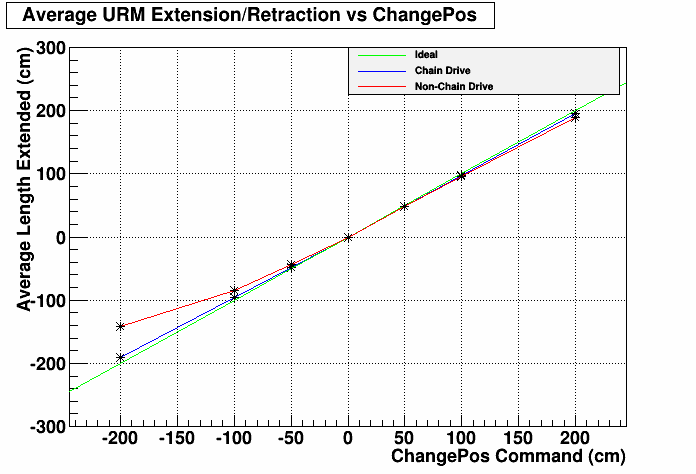
\includegraphics[height=8cm]{Newumb1}
                \caption{Displays a graph generated in ROOT showing the relationship between measured and requested length for both Chain and Non Chain Drive systems with LAB.}
				\label{fit1}
        \end{figure}

        \begin{figure}[H]
                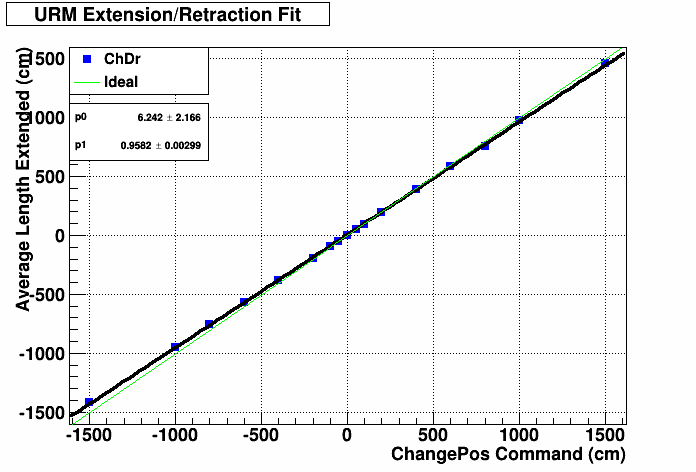
\includegraphics[height=8cm]{big}
                \caption{Displays a graph generated in ROOT showing the relationship between measured and requested length for a chain drive system during longer runs with LAB.}
                \label{fit2}
        \end{figure}

\subsection{Run Consistency}
The slippage of the umbilical on the main drive pulley was reduced by integrating a chain drive system. The consistency of this reduction was also tabulated using ROOT. This was completed by converting all slippage into a percent value. The values of all the runs for a particular set of conditions where tabulated into a histogram to gage the consistency of the chain drive system for both long and short runs during LAB application which are shown in both figures \ref{con1} and \ref{con2}. 

    \begin{figure}[h]
                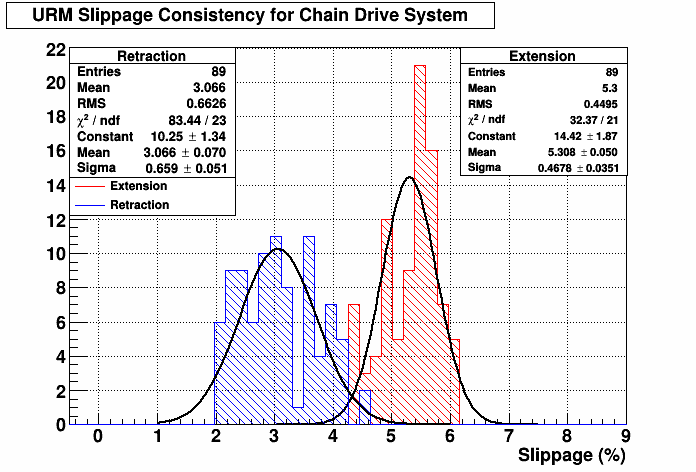
\includegraphics[height=8cm]{fdat1}
                \caption{Displays a graph generated in ROOT showing the consistency of the Chain Drive system with LAB for ChangePos$\pm$(50-1500) }
				\label{con1}
        \end{figure}

        \begin{figure}[h]
                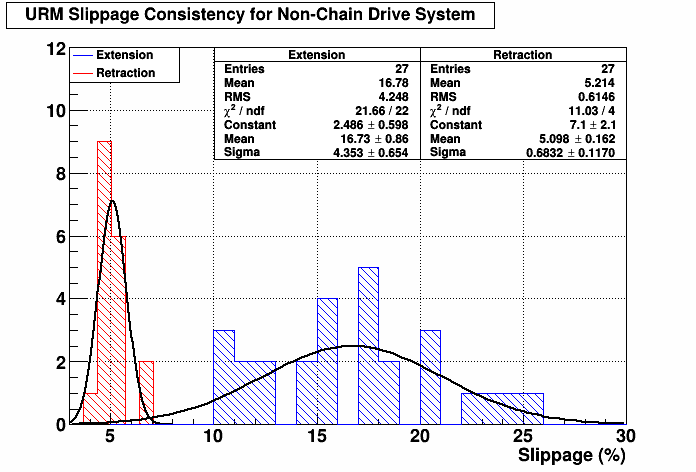
\includegraphics[height=8cm]{fdat2}
                \caption{Displays a graph generated in ROOT showing the consistency of the Non-Chain Drive system with LAB.}
                \label{con2}
        \end{figure}
        
In addition the consistencies of the manually measured values and optical measured values are displayed in figure \ref{op}. These plots shows the consistences of both retracted and extension runs with both the manual and optical method which allows for a validation of the rotary optical sensor. In both cases the optical sensor tends to show slippage being about 1\% less than manually measured values.
        

       
        \begin{figure}[H]
                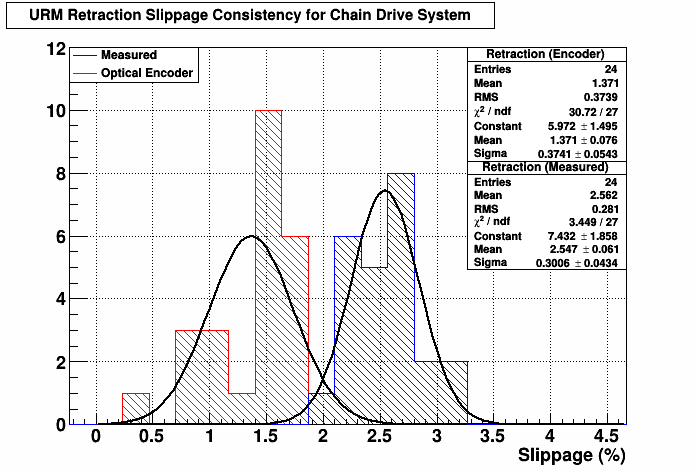
\includegraphics[height=8cm]{fdat3}
                \caption{Shown above are slippage consistences for both manual and optical methods of length change detection during LAB runs for ChangePos$\pm$(50-400)}
				\label{op}
        \end{figure}%
       
        \begin{figure}[H]
                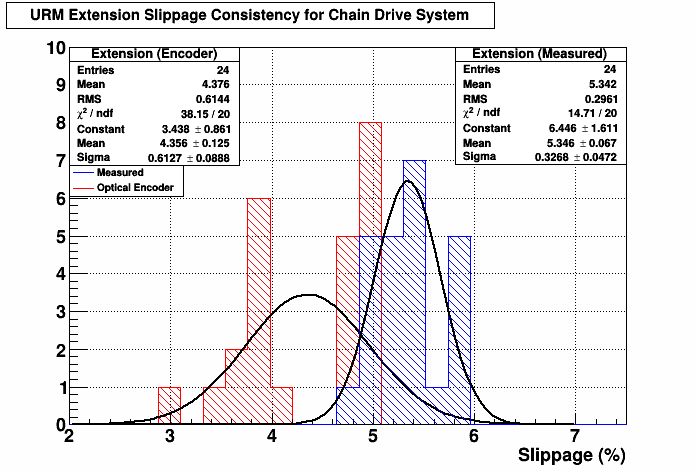
\includegraphics[height=8cm]{fdat4}
                \caption{Shown above are slippage consistences for both manual and optical methods of length change detection during LAB runs for ChangePos$\pm$(50-400)}
                \label{op2}
        \end{figure}
        


\subsection{Conclusions}
After initial testing its clear that driving the big guide pulley via a chain drive system produces significant and consistence slippage reduction in both extension and retraction phases. For extension phases slippage has been on average reduced from 16.7\% down to 5.3\% and for retraction from 5.2\% down to 3.1\%. Not only has the slippage been reduced consistently but the asymmetry between the phases has been significantly reduced. It is my recommendation that future URMs implement appropriate mechanisms to drive one or both guide pulleys in order to significantly reduced slippage. 
\newpage
\section{Future Implementations}
During the scintillation phase new URM will be required for LAB compatibility and to reduce debilitating backgrounds. Proposed designs for the new drive assembly makes integration of a drive system difficult without significant modifications. We have proposed a two of ideas in order to help designers painlessly integrate the drive system.
\subsection{Flex Drive}
\begin{figure}[H]
                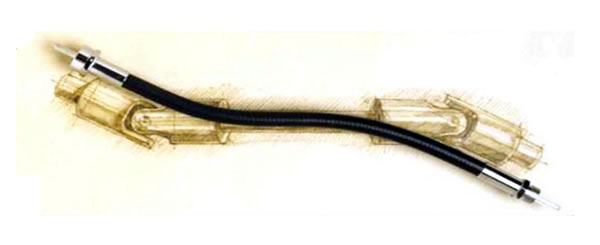
\includegraphics[height=2.5cm]{ag2}
                \caption{Shows picture of a flexible drive shaft \cite{p1}}
				\label{flex}
        \end{figure}
A adaptation of a flexible drive system (figure \ref{flex}) has be proposed as a possible solution for a painless implementation which is displayed in figure \ref{cadf}. The system consists of a gear reduction box which can be easily attached to the side of the motor box (granted the main shaft is slightly extended). From this gear box will run a stainless steel flexible drive shaft which will be encased in a low radon, LAB compatible external casing. 
    \begin{figure}[H]
                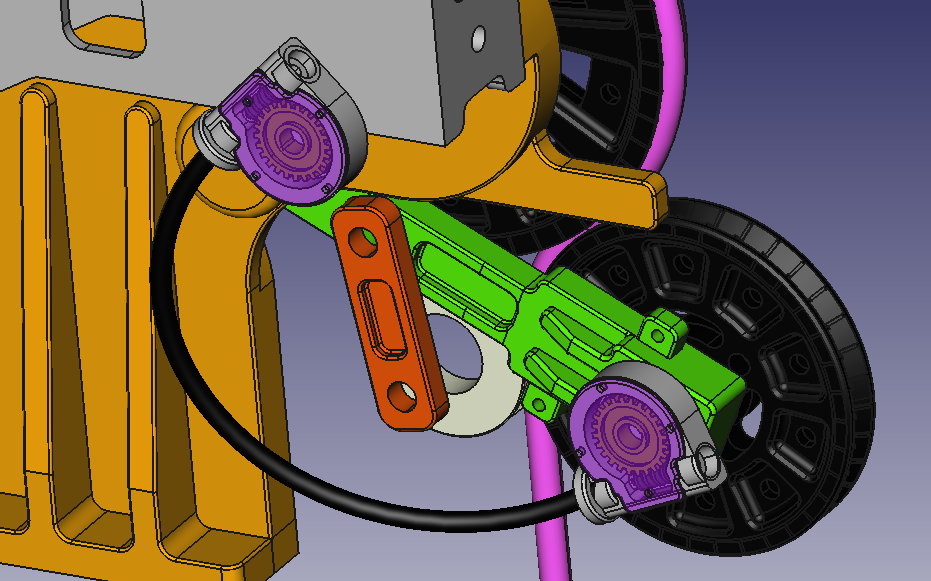
\includegraphics[height=8cm]{newurm1}
                \caption{Displays a design generated using FreeCAD of the implementation of a flex drive system.}
				\label{cadf}
        \end{figure}
        This will connect to another reduction box which will be mounted on a new swing-arm (figure \ref{con2}) which will enable the big guide pulley to be driven. The system complies with space restrictions and requires little modification to the original design. However there is concern on the robustness of the flex drive as the torque requirements for driving the pulley are not known. A tygothane tube can be mounted over the outer casing conforming to the LAB requirements however also finding low radon emanating outer casing will be difficult to find/manufacture.

        \begin{figure}[H]
                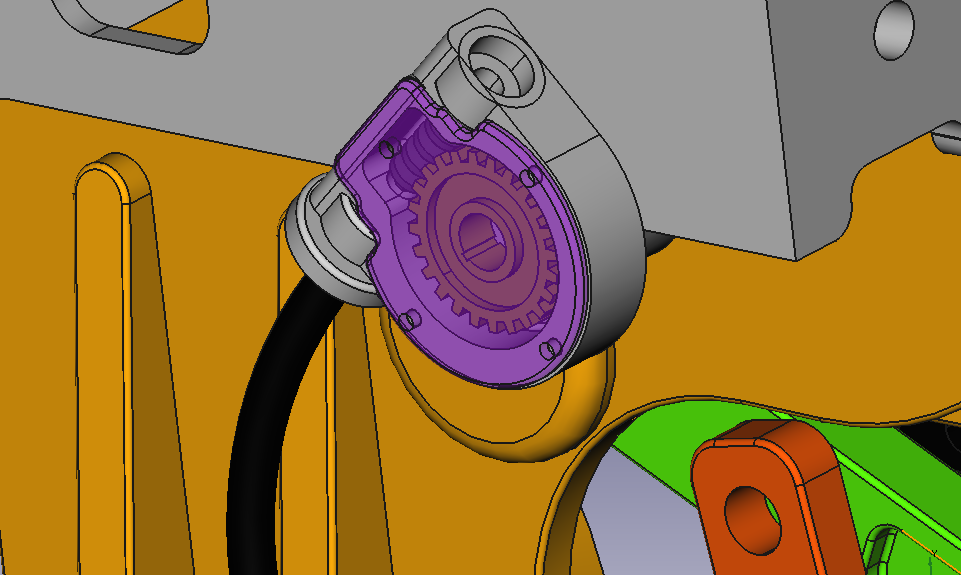
\includegraphics[height=9cm]{newurm3}
                \caption{Displays a design generated using FreeCAD of the implementation of a flex drive system.}
                \label{con2}
        \end{figure}
        
        A hybrid of a gear/chain drive system has be proposed as a possible solution for a painless implementation which is displayed in figure \ref{cadc} and \ref{cadc2}. The system consists of a gear  box which can be easily attached below the motor box and a sprocket can be mounted on the main shaft if its slightly extended. The sealed gear box will contain the appropriate reduction which will drive an additional sprocket which will connect the gear box with a sprocket mounted on the guide pulley shaft. The location of the gear box is chosen to center a sprocket over the pivot point of the swing-arm to prevent chain stretch.  
    \begin{figure}[H]
                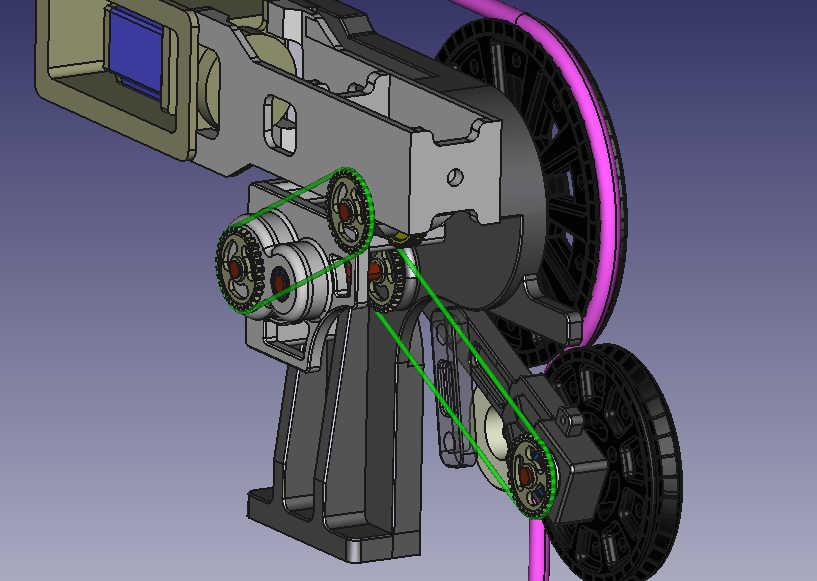
\includegraphics[height=9cm]{URM1}
                \caption{Displays a design generated using FreeCAD of the implementation of a gear/chain drive system.}
				\label{cadc}
        \end{figure}
         The system complies with space restrictions and requires little modification to the original design. This system in contrast to the flex drive system would be able to meet necessary torque requirements. However the addition of a gearbox adds the amount of bearings used in the URM which could significantly increase background. In addition there is also the concern of finding/constructing a chain that would meet background requirements

        \begin{figure}[H]
                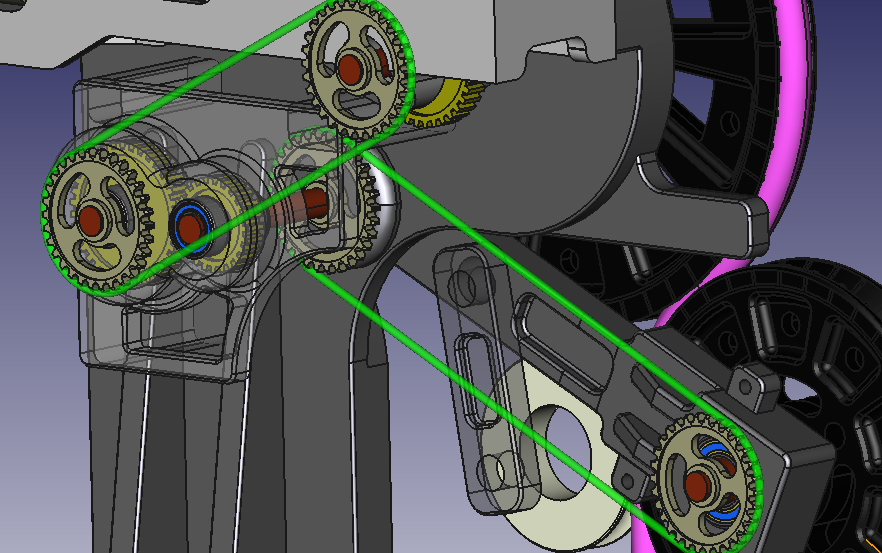
\includegraphics[height=9cm]{URM2}
                \caption{Displays a design generated using FreeCAD of the implementation of a gear/chain drive system.}
                \label{cadc2}
        \end{figure}
        
\subsection{Next Steps}
A summary of possible future steps/goals: Investigate the possible improvements of driving smaller guide pulley, Complete more accurate LAB applications system, Investigate alternative means of Implementing Drive System to new URM design.



\newpage

\appendix
\section{\\ROOT Code } \label{App:Appendix}
\begin{verbatim}
{
TCanvas *c1 = new TCanvas("c1","URMgraph",200,10,700,500);
	 c1->SetFillColor(10);
	 c1->SetGrid();
	 c1->GetFrame()->SetFillColor(10);
	 c1->GetFrame()->SetBorderSize(12);  
//********************************************************************
// A 1D histogram
TH1D *myHist = new TH1D("Retraction","URM Retraction Slippage Consistency",50,-0.5,9);
//read data from text then fill bins in 1st hist
Float_t         z;
FILE *out;
out=fopen("URMhistdata2","r"); 
	while(!feof(out))
	{
	fscanf(out,"%f",&z); 
	myHist->Fill(z*100.); 
	} 
fclose(out);
//new fit for 1st hist
TF1 *myfit = new TF1("fitf","gaus");
fitf->SetLineWidth(2);
fitf->SetLineColor(1);
//Histogram settings
myHist->GetXaxis()->SetTitle("Slippage (%)");
myHist->SetLineColor(4);
myHist->SetFillColor(4);
myHist->SetFillStyle(3005);
//********************************************************************
//Second 1D histogram
TH1D *myHist2 = new TH1D("Extension","URM Slippage Consistency for Chain Drive System",50,-0.5,9);  
//read data from text then fill bins for second hist
Float_t         z;
FILE *out;
out=fopen("URMhistdata1","r"); 
	while(!feof(out))
	{
	fscanf(out,"%f",&z); 
	myHist2->Fill(z*100.); 
	} 
fclose(out);
//create second fit for second hist
TF1 *myfit2 = new TF1("fitf2","gaus");
fitf2->SetLineWidth(2);
fitf2->SetLineColor(1);
// 2nd Histogram settings
myHist2->GetXaxis()->SetTitle("Slippage (%)");
myHist2->SetLineColor(2);
myHist2->SetFillColor(2);
myHist2->SetFillStyle(3005);
//********************************************************************
//Draw Histograms and Fits
myHist2->Fit("fitf","LL","",3,7.5);
gStyle->SetOptFit();
myHist->Fit("fitf","LL","",1,6);
gStyle->SetOptFit();
myHist2->Draw();
myHist->Draw("SAME");
//Draw Legend
leg = new TLegend(0.1,.9,0.3,.85);
leg->AddEntry(myHist2,"Extension","l");
leg->AddEntry(myHist,"Retraction","l");
leg->SetFillColor(0);
leg->Draw();
return c1;
}
\end{verbatim}


\newpage



\begin{thebibliography}{99} % Beamer does not support BibTeX so references must be inserted manually as below
\bibitem[Garcia, 2014]{picfsk} Lawrence Garcia (2014)
\newblock Umbilical Tests and Detector Data Analysis


\bibitem[Maneira, 2013]{p1} Jose Maneira, Rui Alves (2013)
\newblock URM design for SNO+, LIP-Coimbra

\end{thebibliography}


%%% End document
\end{document}